%%*************************************************************************
%% Technische Hochschule Ingolstadt 
%%
%%  
%% Mostly based on Prof. Dr.-Ing. Munir Georges' 2021 template.
%% Original starting code base was obtained from Jonas Wurst's template.
%%
%% 
%%
%% Zur Verwendung für Seminararbeiten
%% an der Technischen Hochschule Ingolstadt
%% Fakultät Informatik 
%%*************************************************************************
\documentclass[11pt,titlepage,a4paper]{article}
\usepackage[utf8]{inputenc}
%\usepackage[ngerman]{babel}  %%<===== Comment out this line iff you write in English.
\usepackage[inner=3.2cm,outer=2.8cm]{geometry}
\usepackage{algorithmic}
\usepackage{listings}
\usepackage{longtable}
\usepackage{float}
\usepackage{fancyhdr,lipsum}
\usepackage{lmodern}
\usepackage[T1]{fontenc}
\usepackage{amsmath,bm}
\usepackage{amsfonts}
\usepackage{amssymb}
\usepackage{fixmath}
\usepackage{amsbsy}
\usepackage{units}
\usepackage{hhline}
\usepackage{titling}
\usepackage{blindtext}
\usepackage{multirow}
\usepackage[pdftex]{graphicx}
\usepackage[pdftex]{xcolor}
\usepackage{lastpage}
\usepackage{afterpage}
\usepackage{hyperref}

%%*************************************************************************
%% Technische Hochschule Ingolstadt 
%%
%% Copyright (c) 2022 Prof. Dr. Christian Seidel   
%% Mostly based on Prof. Dr.-Ing. Munir Georges' 2021 style file.
%% Original starting code base was obtained from Jonas Wurst's template.
%%
%% christian.seidel@thi.de
%%
%% Zur Verwendung für Seminararbeiten
%% an der Technischen Hochschule Ingolstadt
%% Fakultät Informatik 
%%*************************************************************************

\fancyhf{}

\renewcommand{\headrulewidth}{0.1pt}
%\fancyhead[RO]{\nouppercase{\rightmark}}
\fancyhead[RO]{
\includegraphics[width=1cm]{thi_logo_wb_RGB.png} }
\raggedbottom
\fancypagestyle{plain}{%
  \fancyhf{}%
  \renewcommand{\headrulewidth}{0pt}%
  \fancyhf[lef,rof]{\thepage}%
}

\makeatletter
\def\cleardoublepage{\clearpage\if@twoside \ifodd\c@page\else
	\hbox{}
	\vspace*{\fill}
	\begin{center}
	\end{center}
	\vspace{\fill}
	\thispagestyle{empty}
	\newpage
	\if@twocolumn\hbox{}\newpage\fi\fi\fi}
\makeatother

\clearpage{\pagestyle{empty}\cleardoublepage}
\pagestyle{fancy}
\setlength{\headheight}{25pt}
\renewcommand{\sectionmark}[1]{\markright{\thesection.\ #1}}

\linespread{1.3}

\makeatletter
\def\@subtitle{\@latex@warning@no@line{No \noexpand\subtitle given}}
\def\subtitle#1{\gdef\@subtitle{#1}}
\def\subject#1{\gdef\@subject{#1}}
\def\@affiliation{\@latex@warning@no@line{No \noexpand\affiliation given}}
\def\affiliation#1{\gdef\@affiliation{#1}}
\def\@supervisor{\@latex@warning@no@line{No \noexpand\supervisor given}}
\def\supervisor#1{\gdef\@supervisor{#1}}
\def\supervisorAffiliation#1{\gdef\@supervisorAffiliation{#1}}
\def\maketitle{
    \begin{titlepage}
    \hfill 
\includegraphics[clip=,scale=.35]{thi_logo_wb_RGB.png}
  \vspace*{6ex}
	\begin{center}
		{\LARGE \textsc{Technische Hochschule Ingolstadt}} \\[4ex]
		{\Large Fakultät Elektro- und Informationstechnik\\
		Master's degree AI Engineering of Autonomous Systems\\}
	\end{center}
  \vspace*{3ex}
  \begin{center}
    {\Huge \textbf{~
    \@title} }
  \end{center}
  \vspace*{8ex}
  \begin{center}
  	{\huge \textsc{\@subtitle}\\[3ex] }
    {\Large \@author }
  \end{center}
    \vspace*{15ex}
	\begin{flushleft}
        {\large
		\begin{tabular}{ r l }
         Supervisor: & Prof. Dr. Jürgen Bock \\ 
         Date: & \today
        \end{tabular}
        }
	\end{flushleft}	
    \end{titlepage}%
}
\lhead{\@title}
\renewcommand{\footrulewidth}{0.4pt}% Default \footrulewidth is 0pt
\rfoot{ \thepage}
% \lfoot{ \@author}
\cfoot{ \nouppercase{\rightmark} }

\makeatother

\definecolor{codegreen}{rgb}{0,0.6,0}
\definecolor{codegray}{rgb}{0.5,0.5,0.5}
\definecolor{codepurple}{rgb}{0.58,0,0.82}
\definecolor{backcolour}{rgb}{1.0,1.0,1.0}

\lstdefinestyle{mystyle}{
    backgroundcolor=\color{backcolour},   
    commentstyle=\color{codegreen},
    keywordstyle=\color{magenta},
    numberstyle=\tiny\color{codegray},
    stringstyle=\color{codepurple},
    basicstyle=\ttfamily\footnotesize,
    breakatwhitespace=false,         
    breaklines=true,                 
    captionpos=t,                    
    keepspaces=true,                 
    numbers=left,                    
    numbersep=5pt,                  
    showspaces=false,                
    showstringspaces=false,
    showtabs=false,                  
    tabsize=2
}

\lstset{style=mystyle}


\newcommand\blankpage{%
    \null
    \thispagestyle{empty}%
    \addtocounter{page}{-1}%
    \newpage}
\affiliation{Technische Hochschule Ingolstadt}
\supervisor{Prof. Dr. Jürgen Bock, Maximilian-Peter Radtke}
\supervisorAffiliation{Technische Hochschule Ingolstadt}
\date{\today}
\subtitle{Seminar paper}



\DeclareMathOperator*{\argmin}{arg\,min}
\DeclareMathOperator*{\argmax}{arg\,max}
\renewcommand{\arraystretch}{1.2}

%%%%%%%%%%%%%%%%%%%%%%%%%%%%%%%%%%%%%%%%%%%%%%%%%%%%%%%%%% 
\title{Software Engineering Team Project: Flash Card Web Application} %% <= Titel eintragen
\author{Bükülmez Gizem} %% <= Name eintragen

\begin{document}
%    \afterpage{\blankpage} % optional
    \maketitle

%%%%%%%%%%%%%%%%%%%%%%%%%%%%%%%%%%%%%%%%%%%%%%%%%%%%%%%%%% 
    
%    \afterpage{\blankpage} % optional
    \tableofcontents
    \thispagestyle{empty}
    \newpage
    \setcounter{page}{1}
    
%%%%%%%%%%%%%%%%%%%%%%%%%%%%%%%%%%%%%%%%%%%%%%%%%%%%%%%%%% 
    %\usepackage{tocbibind} % İçindekiler kısmını otomatik olarak ekler

\newpage

\section{Introduction}

Flash cards have long been used as an effective way to help people learn and remember information through active recall and spaced repetition techniques. The advancement of digital technologies has made it possible to use these flashcards as interactive and fun applications.

Software testing is one of the most critical components of the software development process. A proper testing strategy is necessary to verify that the software works as expected and to detect potential bugs at an early stage. In this paper, the pytest library and the process of testing a flask application will be discussed in detail. It will also explain step by step how a flask application is tested. In this framework, the importance of effective testing strategies to ensure the quality and reliability of flash card applications will be emphasized.

\section{System Design}
The Flash Card application is designed using a client-server architecture. In this architecture, server-side operations are managed by the Flask framework. Flask performs critical server-side operations such as user authentication, flash card management and game functionality. Data is stored in two JSON files, \texttt{user\_data.json} containing user information and \texttt{data.json} containing flash card details. The client side is built using Bootstrap, HTML and JavaScript to provide a responsive and interactive experience for the user. This structure allows users to interact with flash cards easily and effectively.

            \begin{figure}[H]
                \centering
                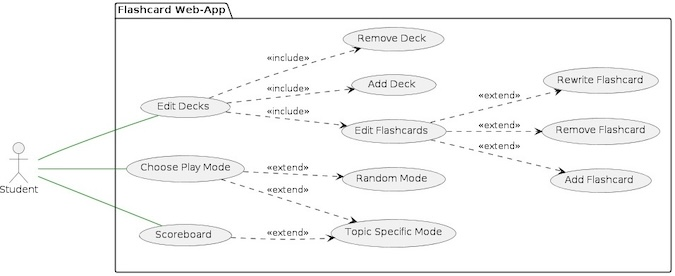
\includegraphics[width=0.9\textwidth]{UCD.jpeg}
                \caption{Flashcard Web Application Use Case Diagram}
                \label{fig:FlashcardWebApplicationUseCaseDiagram}
            \end{figure}\newpage


\section{Development}

\subsection{Role}
As a Tester, my task was to gain in-depth knowledge about the software architecture and application to ensure that the created software architecture works flawlessly. I created a test case by developing a new test architecture to match this architecture. However, during this process, I encountered some difficulties in the 'flask8' section and encountered pipeline errors. Fortunately, with the changes I made to the test architecture, I was able to overcome these challenges and make the application more reliable and robust.

\subsection{Flash App}
flask is a micro web framework written in Python. Thanks to its simple and flexible structure, it enables fast development of web applications. flask applications are usually defined in the \texttt{app.py}  file and serve different endpoints through various routes.

\subsection{What is Pytest?}
Pytest is a testing framework written in Python programming language. It allows users to easily write tests with its simple, scalable and extensible structure. Pytest automatically discovers and runs your tests. It also allows you to easily manage setup and teardown processes.

\subsection{Creating the Test File}

In our test file, we will use pytest to test various functions and routes of our flask application. The file containing our tests is usually named \texttt{test\_*.py} and is located in the application root directory or in a directory called \texttt{tests}.

Below you can find a detailed description of a \texttt{test\_routes.py} file containing the tests of our flask application.


\paragraph{Required Imports}
First, we import the necessary libraries and modules:

\begin{lstlisting}[language=Python]
import pytest
from app import app
from app.models import User, Card
\end{lstlisting}\newpage


\subsubsection{Test Client and User Preparation}

\paragraph{Test Client}
We create a test client to use in our tests. The test client allows us to run our application in test mode:

\begin{lstlisting}[language=Python]
@pytest.fixture
def client():
    app.config['TESTING'] = True
    app.config['WTF_CSRF_ENABLED'] = False
    with app.test_client() as client:
        with app.app_context():
            # setup database and other initializations
            yield client
\end{lstlisting}

Here we set \texttt{app.config} to test mode and disable CSRF protection. We create a test client with \texttt{app.test\_client() and provide the application context with \texttt{app.app\_context()}.
}

\paragraph{New User}
We create a new user to use in our tests:

\begin{lstlisting}[language=Python]
@pytest.fixture
def new_user():
    user = User(username='test_user', email='test@example.com')
    user.set_password('password')
    users = User.load_users()
    users[user.username] = user
    User.save_users(users)
    return user
\end{lstlisting}

This function creates a user from the User model and loads and saves this user.

\paragraph{Logging in}
We define a fixture that performs the login process with the new user:

\begin{lstlisting}[language=Python]
@pytest.fixture
def login(client, new_user):
    response = client.post('/login', data=dict(
        username=new_user.username,
        password='password'
    ), follow_redirects=True)
    assert response.status_code == 200
    return response
\end{lstlisting}

This fixture logs in with the newly created user and verifies that the login was successful.\newpage

\subsection{Test Functions}

\paragraph{User Registration Test}
We create a test function that tests the user registration function:

\begin{lstlisting}[language=Python]
def test_register(client):
    response = client.get('/register')
    assert response.status_code == 200
    response = client.post('/register', data=dict(
        username='test_user2',
        email='test2@example.com',
        password='password',
        password2='password'
    ), follow_redirects=True)
    assert response.status_code == 200
\end{lstlisting}

This function sends GET and POST requests to the \texttt{/register} route and checks the status code.

\paragraph{Login Test}
We create a test function that tests the login function:

\begin{lstlisting}[language=Python]
def test_login(client, new_user):
    response = client.get('/login')
    assert response.status_code == 200
    response = client.post('/login', data=dict(
        username='test_user',
        password='password'
    ), follow_redirects=True)
    assert response.status_code == 200
\end{lstlisting}

This function sends GET and POST requests to the \texttt{/login} route and checks if the login was successful.

\paragraph{Logout Test}
We create a test function that tests the output function after input:

\begin{lstlisting}[language=Python]
def test_logout(client, login):
    response = client.get('/logout', follow_redirects=True)
    assert response.status_code == 200
\end{lstlisting}

This function sends a GET request to the \texttt{/logout} route and checks if the logout was successful.\newpage

\paragraph{All Cards Test}
We create a test function that tests the route where all cards are listed:

\begin{lstlisting}[language=Python]
def test_all_cards(client, login):
    response = client.get('/all_cards')
    assert response.status_code == 200
\end{lstlisting}

This function sends a GET request to the \texttt{/all\_cards} route and checks if the response is successful.

\paragraph{Home Page Test}
We create a test function that tests the home page route:

\begin{lstlisting}[language=Python]
def test_index(client, login):
    response = client.get('/')
    assert response.status_code == 200
\end{lstlisting}

This function sends a GET request to the home page route and checks if the response is successful.

\paragraph{Post Login Test}
After logging in, we create a test function that tests the redirected page:

\begin{lstlisting}[language=Python]
def test_post_login(client, login):
    response = client.get('/post_login')
    assert response.status_code == 200
\end{lstlisting}

This function sends a GET request to the \texttt{/post\_login} route and checks if the response is successful.

\paragraph{Post Entry Action Test}
We create a test function that tests an action performed after logging in:

\begin{lstlisting}[language=Python]
def test_post_login_action(client, login):
    response = client.post('/post_login_action', data=dict(action="start_game"), follow_redirects=True)
    assert response.status_code == 200
\end{lstlisting}

This function sends a POST request to the \texttt{/post\_login\_action} route and checks if the response is successful.\newpage

\paragraph{Topic Based Initialization Test}
We create a test function that tests the initialization function based on a specific topic:

\begin{lstlisting}[language=Python]
def test_start_by_topic(client, login):
    response = client.get('/start_by_topic')
    assert response.status_code == 200
\end{lstlisting}

This function sends a GET request to the \texttt{/start\_by\_topic} route and checks if the response is successful.

\paragraph{New Card Creation Test}
We create a test function that tests the function to create a new card:

\begin{lstlisting}[language=Python]
def test_new_card(client, login):
    response = client.get('/cards/new')
    assert response.status_code == 200

    response = client.post('/cards/new', data=dict(
        topic='Test Topic',
        question='Test Question',
        hint='Test Hint',
        answer='Test Answer'
    ), follow_redirects=True)
    assert response.status_code == 200

    % Check if the card was actually added
    cards = Card.load_cards()
    assert any(card.topic == 'Test Topic' and card.question == 'Test Question' for card in cards)
\end{lstlisting}

This function sends GET and POST requests to a new card creation page and checks if the card was created successfully.

\paragraph{Showing Cards Test}
We create a test function that tests the page where all the cards are listed:

\begin{lstlisting}[language=Python]
def test_show_cards(client, login):
    response = client.get('/all_cards')
    assert response.status_code == 200
\end{lstlisting}

This function sends a GET request to the \texttt{/all\_cards} route and checks if the response is successful.\newpage

\paragraph{Game Launch Test by Topic}
We create a test function that tests the game initialization function based on a specific topic:

\begin{lstlisting}[language=Python]
def test_start_game_by_topic(client, login):
    % First add a card to ensure there's at least one card
    client.post('/cards/new', data=dict(
        topic='TestTopic',
        question='TestQuestion',
        hint='TestHint',
        answer='TestAnswer'
    ))
    response = client.get('/start_game_by_topic/TestTopic')
    assert response.status_code == 200
\end{lstlisting}

This function adds a card before starting a game based on a specific topic and then sends a GET request to the corresponding route.



\paragraph{Test Fetching Card Topic}
We create a test function that tests the function to fetch cards of a given topic:

\begin{lstlisting}[language=Python]
def test_get_card_topic(client, login):
    response = client.get('/cards/topic/test_topic')
    assert response.status_code == 200

\end{lstlisting}

This function sends a GET request to the \texttt{/cards/topic/test\_topic} route and checks if the response is successful.

\paragraph{Card Editing Test}
We create a test function that tests an existing card editing function:

\begin{lstlisting}[language=Python]
def test_edit_card(client, login):
    # First, add a card
    client.post('/cards/new', data=dict(
        topic='EditTopic',
        question='EditQuestion',
        hint='EditHint',
        answer='EditAnswer'
    ))
    # Get the id of the newly added card
    cards = Card.load_cards()
    card_id = max(card.id for card in cards)
    # Edit the card
    response = client.post(f'/cards/{card_id}', data=dict(
        topic='EditedTopic',
        question='EditedQuestion'
    ), follow_redirects=True)
    assert response.status_code == 200
    # Check if the card was actually edited
    updated_cards = Card.load_cards()
    edited_card = next((card for card in updated_cards if card.id == card_id), None)
    assert edited_card is not None
    assert edited_card.topic == 'EditedTopic'
    assert edited_card.question == 'EditedQuestion'

\end{lstlisting}

This function edits an existing card and checks if the edit was successful.


\paragraph{Card Delete Test}
We create a test function that tests the function to delete an existing card:

\begin{lstlisting}[language=Python]
def test_delete_card(client, login):
    # First, add a card
    client.post('/cards/new', data=dict(
        topic='DeleteTopic',
        question='DeleteQuestion',
        hint='DeleteHint',
        answer='DeleteAnswer'
    ))
    # Get the id of the newly added card
    cards = Card.load_cards()
    card_id = max(card.id for card in cards)
    # Delete the card
    response = client.post(f'/cards/{card_id}/delete', follow_redirects=True)
    assert response.status_code == 200
    # Check if the card was actually deleted
    updated_cards = Card.load_cards()
    assert all(card.id != card_id for card in updated_cards)


\end{lstlisting}

This function deletes an existing card and checks if the deletion was successful.\newpage

\paragraph{Scoreboard Test}
We create a test function that tests the scoreboard sheet:

\begin{lstlisting}[language=Python]
def test_scoreboard(client, login):
    response = client.get('/scoreboard')
    assert response.status_code == 200

\end{lstlisting}

This function sends a GET request to the /scoreboard route and checks if the response is successful.

\section{Measuring the Performance of a Flask Application with Load Testing}

Performance testing is an important type of testing used to analyze how an application behaves under certain loads. These tests are performed to determine how the application performs under high loads, response times and how resilient the system is. Locust is a popular performance testing tool used for this purpose. In this paper, we will cover how to performance test a flask application using Locust and create an example scenario step by step.

\subsection{What is Locust?}
Locust is an open source performance testing tool used to perform load testing of a web application. By simulating the user's behavior, Locust puts a certain load on the application for a certain period of time and evaluates the performance of the application.

\subsection{Performance Testing of flask Application}

\subsubsection{Test Scenario}
In this performance test, we will simulate users registering, logging in and adding a new card. These steps will simulate the basic interactions of a user and evaluate the performance of the application under these actions.
\subsection{Installing the Required Libraries}

            \begin{figure}[H]
                \centering
                
\includegraphics[width=0.65\textwidth]{image.png}
                \caption{Installing locust}
                \label{fig:InstallingLocust}
            \end{figure}

\subsection{Creating Locust Test File}
In order to test performance with Locust, we create a test file. In this file, we will write code to simulate user behavior. Here is a sample Locust test file:

\begin{lstlisting}[language=Python]
from locust import HttpUser, task, between

class UserBehavior(HttpUser):
    wait_time = between(5, 9)  # time between requests
    host = "http://127.0.0.1:5000"  # base URL

    @task
    def register_login_add_card(self):
        # Register a new user
        response = self.client.post('/register', data=dict(
            username='test_user3',
            email='test3@example.com',
            password='password',
            password2='password'
        ))

        # check registration was successful by looking at response status
        if response.status_code == 200:
            # Log in with the new user credentials
            login_response = self.client.post('/login', data=dict(
                username='test_user3',
                password='password'
            ))

            # if login was successful
            if login_response.status_code == 200:
                # add new card
                self.client.post("/cards/new", data=dict(
                    topic="Science",
                    question="What is photosynthesis?",
                    hint="Hint: It involves plants.",
                    answer="The process by which plants convert light energy into chemical energy."
                ))


\end{lstlisting}\newpage



\paragraph{Description of Test Scenario}
- \texttt{wait\_time}: Sets the waiting time between requests. This is a random wait time between 5 and 9 seconds.
- host: The base URL of the application to be tested.
- \texttt{register\_login\_add\_card method}: A task that simulates user behavior. This task first registers a new user, then logs in with that user and finally adds a new card.

\paragraph{Running the Test}

You can use the following command to run the Locust test:

locust -f locustfile.py

This command will launch the Locust web interface. You can access the Locust interface and start the test by going to http://localhost:8089 in your web browser.

\paragraph{Evaluation of Test Results}

In the Locust interface, you can start the test by specifying the number of users and the test duration. During and after the test, Locust provides you with various metrics. These metrics include:

- Number of requests
- Number of successful requests
- Error rate
- Average response time
- Maximum response time
- Median response time

These metrics help you assess the performance of your application and identify potential performance bottlenecks.


\section{Conclusion}

In this article, we focused on testing Flask applications from both software testing and performance testing perspectives. First, we went through step-by-step how to test Flask applications using pytest. We created test files, defined the necessary fixtures, and wrote tests of various functions and routes. This process highlighted the use of pytest, a powerful tool that is critical for improving quality and reliability in the software development process.

Next, we learned how to perform performance tests of Flask applications using Locust. Performance tests are vital to understand how the application performs under high load and make necessary improvements. Locust's simple and flexible structure made it an ideal tool to run such tests effectively. By regularly running performance tests, we can ensure that the application always performs at its best.\newpage

\section{References}


        \begin{itemize}
        \item [1] Pytest Documentation: \url{https://docs.pytest.org/en/8.2.x/}
        \item [2] Locust Documentation: \url{https://docs.locust.io/en/stable/}
        \item [3] AI Tools - Chat-GPT, I ASK AI: \url{https://iask.ai/}
    \end{itemize}\newpage


\section{Appendix}
%\subsection{Team Discussions}


\section*{Team Discussions}

\subsection*{20.05.2024 - Overview}
\begin{itemize}
    Basic structure of app.\newline
    Tools to be used.\newline
    Work flow and use cases.\newline
\end{itemize}

\subsection*{29.05.2024 - Pre-Implementation Phase-1}
    Creation of task-based system and continuous monitoring in teams.
    Prioritization of tasks and sub-grouping to achieve a fast-paced environment.
    Tools to be used and how to proceed with these:
    \begin{itemize}
        \item Frontend - Angular\newline
        \item Backend - Django\newline
        \item Database - MYSQL\newline
        \item CI/CD and Dockerization
    \end{itemize}
    Coding standards to be followed via documentation.

\subsection*{01.06.2024 - Implementation Phase-1}
    Change in use of tools due to complexity for such a simple app structure:\newline
        Frontend - HTML/CSS/JavaScript\newline
        Backend - Flask\newline
        Database - Text File
    Frontend - How Chat-GPT is very useful in creating bootstrap and playing with JS for creating forms and interaction with UI - we have a current structure of all forms by now.\newline
    Backend - Flask is less complex compared to Django and for such a small-scale application it’s better to go with what is simple and easy to understand - implemented some basic routes such as login/home pages.\newline
    Database - Rather than using MYSQL we can go for simple text files, as we don’t have complex multiple tables to deal with primary key/foreign key. It is easy to manipulate and the learning curve is reduced.

\subsection*{07.06.2024 - Implementation Phase-2}
    Change in use of tools:\newline
    \begin{itemize}
        \item Database - JSON File
    \end{itemize}
    Database - Changed the use of Text file into JSON file which is easy to manipulate and has multiple key and value pairs which helps understand and parse easily in any component of the app - logic for two .json files for users and cards dataset.\newline
    Implemented a basic working app with all initial features.\newline
    Testing started parallelly on modules - unit testing.\newline
    Have a sample implemented overview on CI/CD pipelines for pytest in GitLab.\newline
    Parallelly working on Algorithm for display of cards.


\subsection*{12.06.2024 - Implementation Phase-3}
    Have a working prototype of a fully-fledged app.\newline
    Containerized and tested the app locally on Dockerhub.\newline
    Looking for Improvements and further proceedings.

\subsection*{19.06.2024 - Implementation Phase-4}
    Check for load testing for easy user experience.\newline
    Integrate the initial simple algorithm into the backend.\newline
    Working for further optimization and monitoring.\newline
    Checking for the deployment of the app on any open-source cloud platforms.\newline
    Checking for more complex algorithms to display the most prioritized card.


\subsection*{25.06.2024 - Implementation Phase-4}
    Stick to the basic algorithm - which works better than the complex one.\newline
    Tried to deploy the app on Heroku cloud - facing some difficulty in integration.\newline
    Looking for future works and improvements.



 %% <= Text schreiben
    
%%%%%%%%%%%%%%%%%%%%%%%%%%%%%%%%%%%%%%%%%%%%%%%%%%%%%%%%%% 
\end{document}
